\chapter{Apprentissage profond}
\markboth{Apprentissage profond}{}
\section{Introduction}
    Dans le passé proche , les fonctions de tout type d'ordinateurs est d'executer des programmes qui n'étaient qu'une éxecution des instructions sans pouvoir s'entrainer à apprendre des données et produire de la connaissance sans intervention de l'être humain .
    
    Alors , les experts en mathématiques et informatique ont pu révolutionner le monde d'ordinateurs avec ce qu'on appelle "intelligence artificielle" (IA) , là nous parlons d'un ensemble d'algorithmes qui rendent les machines capables d'imiter l'intelligence humaine (c'est-à-dire machines intelligentes) et avoir des connaissances qui ne peuvent être concluses que par les experts humains .
    
    C'est dans ce contexte là que les experts essaient toujours d'améliorer l'intelligence artificielle par le développement de nouvelles algorithmes et l'amélioration d'autres afin que les machines puissent résoudre des problèmes plus complexes et pouvoir s'entrainer à partir d'une très grande massivité de données (Big data)
 
\subsection{Techniques de l'intelligence aritificielle}
    Comme déja mentionné , l'intelligence artificielle englobe un nombre très important de techniques , on peut citer \cite{artificial_intelligence_vs_machine_learning_vs_deep_learning} \cite{asemi2021intelligent} :
    \begin{itemize}[label=$\bullet$]
    \item Les systèmes experts
    \item L'intelligence artificielle symbolique (IA symbolique)
    \item Les algorithmes génétiques
    \item Les algorithmes évolutionnaires 
    \item La logique floue
    \item Les réseaux bayésiens
    \item les algorithmes de l'apprentissage automatique (qui dominent la plupart des algorithmes d'intelligence artificielle) 
    \end{itemize}

\subsection{Domaines d'application de l'intelligence aritificielle}
    Nous allons citer les domaines d'applications des techniques d'IA autres que l'apprentissage automatique tant que ce dernier est un domaine très vaste :
    \begin{itemize}[label=$\bullet$]
    \item Diagnostic médical, la maintenance industrielle, le support technique, ...(Systèmes experts)
    \item Applications en robotique, planification automatique, jeux, ...(IA symbolique)
    \item Optimisation dans divers domaines tels que la conception de   produits, la planification de tâches, la finance, ...(Algorithmes génétiques et évolutionnaires)
    \item Contrôle de processus industriels, systèmes d'aide à la   décision, système de climatisation, ...(Logique floue)
    \item Diagnostic médical, reconnaissance de formes, modélisation probabiliste, ...(Réseaux bayésiens)
    \end{itemize}

\section{Apprentissage automatique}
    l'apprentissage automatique , aussi connu sous le nom "Machine Learning"(ML) qui fait partie de l'IA , se fonde sur des approches mathématiques et statistiques qui visent à apprendre aux machines à tirer des connaissances des données et à s'améliorer avec l'expérience, au lieu d'être explicitement programmées pour le faire.
    Dans le Machine Learning, les algorithmes sont entraînés à trouver des patterns et des corrélations dans de grands ensembles de données, ainsi qu'à prendre les meilleures décisions et à émettre les meilleures prévisions en s'appuyant sur leur analyse. Avec la pratique, les applications du Machine Learning s'améliorent. \cite{what_is_machine_learning}

     L'un des quatre modèles d'apprentissage automatique peut être utilisé : supervisé, non supervisé, semi-supervisé ou par renforcement. Dans chacun de ces modèles, une ou plusieurs techniques algorithmiques peuvent être appliquées ,tout dépend des ensembles des données qui seront utilisés et de l'objectif visé au niveau des résultats. Par nature, les algorithmes de Machine Learning sont conçus pour classifier des éléments, repérer des patterns, prévoir des résultats et prendre des décisions éclairées. \cite{what_is_machine_learning}

     \begin{figure}[htbp]
     \centering    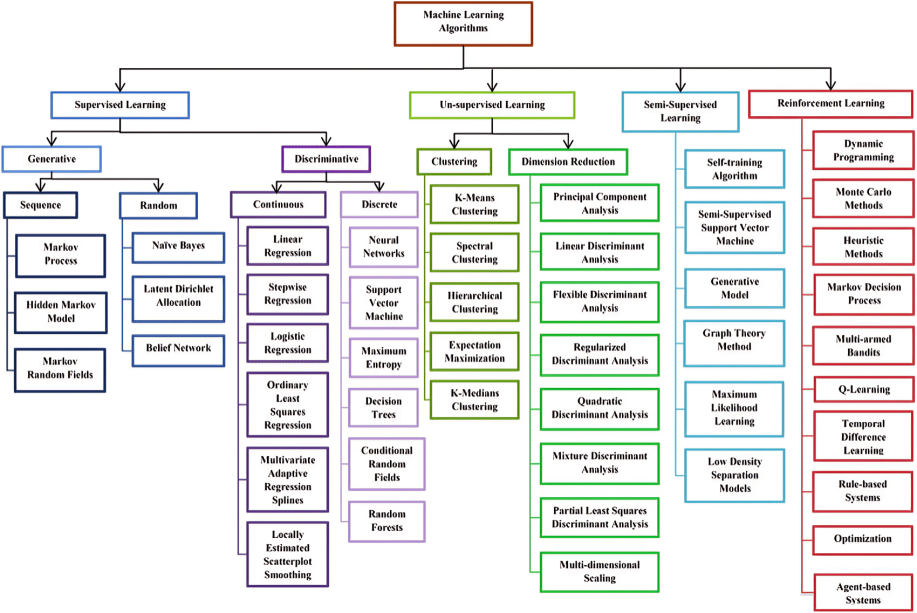
\includegraphics[width=1\textwidth,height=0.5\textheight]{img/Machine_Learning_ML_methods_taxonomy2.png}
     \caption{Techniques d'apprentissage automatique  \cite{sundararajan2021}}
     \label{fig:example2}
     \end{figure}

\subsection{types des techniques d'apprentissage automatique}   
\subsubsection{Apprentissage supervisé(Supervised Learning)}
Nous parlons des algorithmes qui ont besoin d'une supervision humaine qui alimente le dataset (les données à s'entrainer) avec des données de sortie , donc on a une connaissance préalable de ce que les valeurs de sortie pour nos échantillons devraient être \cite{apprentissage_supervise_definition}.Les modèles de l'apprentissage supervisé se composent de paires de données « d'entrée » et « de sortie », dans lesquelles la sortie est étiquetée avec la valeur souhaitée\cite{what_is_machine_learning}.
     \begin{figure}[htbp]
     \centering    
     \includegraphics[width=0.8\textwidth]{supervisé.png}
     \caption{déroulement standard d'un algorithme d'apprentissage supervisé  \cite{apprentissage_supervise_definition}}
     \label{fig:example3}
     \end{figure}

     
Au moyen d'un algorithme, le système compile l'ensemble de ces données d'entraînement et les met en corrélation (mesurer la relation entre une variable dépendante et une ou plusieurs variables indépendantes). Il commence alors à identifier des similarités, des différences et d'autres points de logique, jusqu'à ce qu'il puisse donner par lui-même la réponse à une question.

 
\textbf{Catégories des techniques de l'apprentissage supervisé :} il y a la classification donnée dans la figure 2.1 , et il existe aussi une classification qui est la plus connue dans plusieurs ressources : 

-\textbf{   a.Les algorithmes de régression :}des algorithmes qui cherchent à prédire une valeur continue, une quantité , tels que :
\begin{itemize}[label=$\bullet$]
\item Régression linéaire.
\item Régression polynomiale.
\item Régression Ridge.
\item Régression Lasso.
\item etc ...
\end{itemize}

-\textbf{   b.Les algorithmes de classification :}des algorithmes qui cherchent à prédire une classe/catégorie.
\begin{itemize}[label=$\bullet$]
\item Régression logistique.
\item Machine à vecteurs de support (SVM).
\item Forêt aléatoire.
\item Arbre de décision.
\item K-plus proches voisins (KNN).
\item Naïve Bayes.
\item etc ...
\end{itemize}

\textbf{Applications des techniques d'apprentissage supervisé :}
\begin{itemize}[label={*}]
\item Prédiction de la croissance démographique de la population
\item Détection des des spams ou du courrier indésirable.
\item prévisions météorologiques
\item Prédiction de la hausse/baisse de la valeur de la devise
\item etc ...
\end{itemize}

\vspace{2cm}

\subsubsection{Apprentissage non supervisé(Unsupervised Learning)}
Dans les modèles de cet apprentissage, aucune clé de réponse n'est fournie. La machine étudie les données d'entrée, dont la grande majorité sont non étiquetées et non structurées, et recherche des patterns et des corrélations entre les données pertinentes et accessibles.
Pour nous les humains , plus nous acquérons de l'expérience sur un élément ou un domaine, plus notre capacité à le catégoriser et à le repérer gagne en précision. Dans le cas des machines, « l'expérience » se traduit par le volume de données auxquelles elles ont accès\cite{what_is_machine_learning}. 

     \begin{figure}[htbp]
     \centering    
     \includegraphics[width=0.8\textwidth,height=0.3\textheight]{img/non_supervisé.png}
     \caption{déroulement standard d'un algorithme d'apprentissage non supervisé \cite{apprentissage_supervise_definition}}
     \label{fig:example4}
     \end{figure}



\textbf{Catégories des techniques de l'apprentissage non supervisé :}
 Il existe trois principales catégories d'algorithmes \cite{supervised_vs_unsupervised_learning}:
 
 \textbf{Clustering} : les données non étiquetées sont regroupées à l'aide de techniques de regroupement en fonction de leurs similitudes ou de leurs différences. Par exemple, si une équipe travaille sur la segmentation du marché, l'algorithme de clustering k-moyennes (k-means) attribuera des points de données similaires aux groupes qui représentent un ensemble de paramètres.

 \begin{figure}[htbp]
     \centering    
     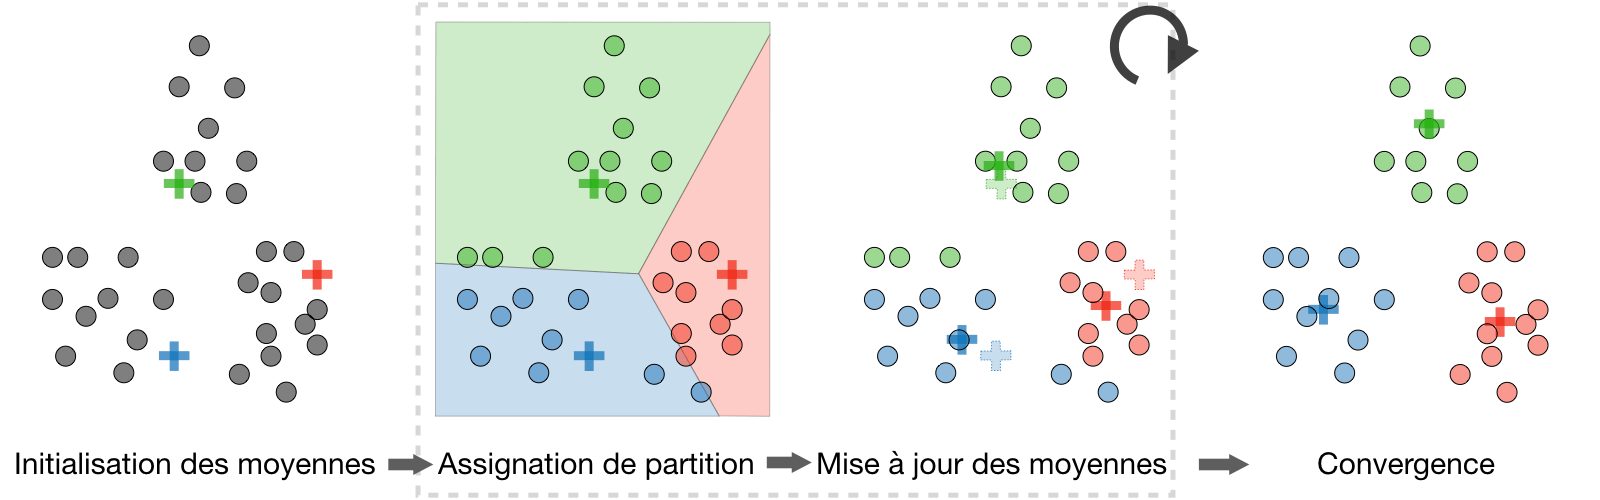
\includegraphics[width=0.9\textwidth,height=0.2\textheight]{k_means_fr.png}
     \caption{étapes de l'algorithme k-means \cite{pense_bete_apprentissage_non_supervise}}
     \label{fig:example5}
     \end{figure}


\textbf{Association} : cette catégorie est intéressante pour trouver des relations entre les variables d'un jeu de données. C'est la technique utilisée pour créer le message de type « les autres clients ont également consulté ». Elle est particulièrement adaptée aux moteurs de recommandation. 

\vspace{1cm}

\textbf{Réduction de la dimensionnalité} : il arrive qu'un jeu de données comporte un nombre de caractéristiques exceptionnellement élevé. La réduction de la dimensionnalité permet de réduire ce nombre sans compromettre l'intégrité des données. Il s'agit d'une technique couramment utilisée avant le traitement des données. Cela sert par exemple à supprimer le bruit d'une image pour améliorer sa qualité.


\begin{figure}[htbp]
     \centering    
     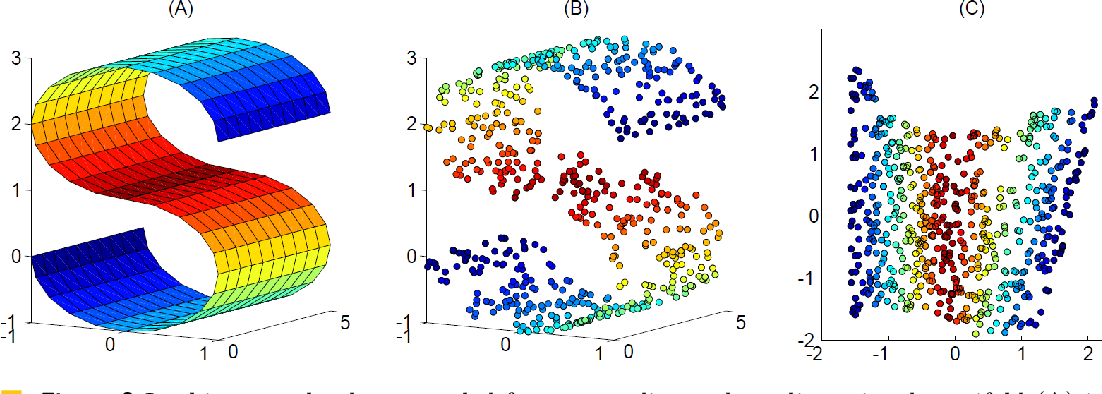
\includegraphics[width=0.8\textwidth]{réduction_de_dimensionalité.png}
     \caption{Exemple de réduction de dimensionalité (3D vers 2D) \cite{reduction_de_dimensionalite}}
     \label{fig:example6}
     \end{figure}

\vspace{1cm}

\textbf{Applications des techniques d'apprentissage non-supervisé :}
\begin{itemize}[label={*}]
\item La reconnaissance faciale.
\item L'analyse de séquences génétiques.
\item Les études de marché.
\item la cybersécurité.
\item etc ...
\end{itemize}

     \begin{figure}[htbp]
     \centering    
     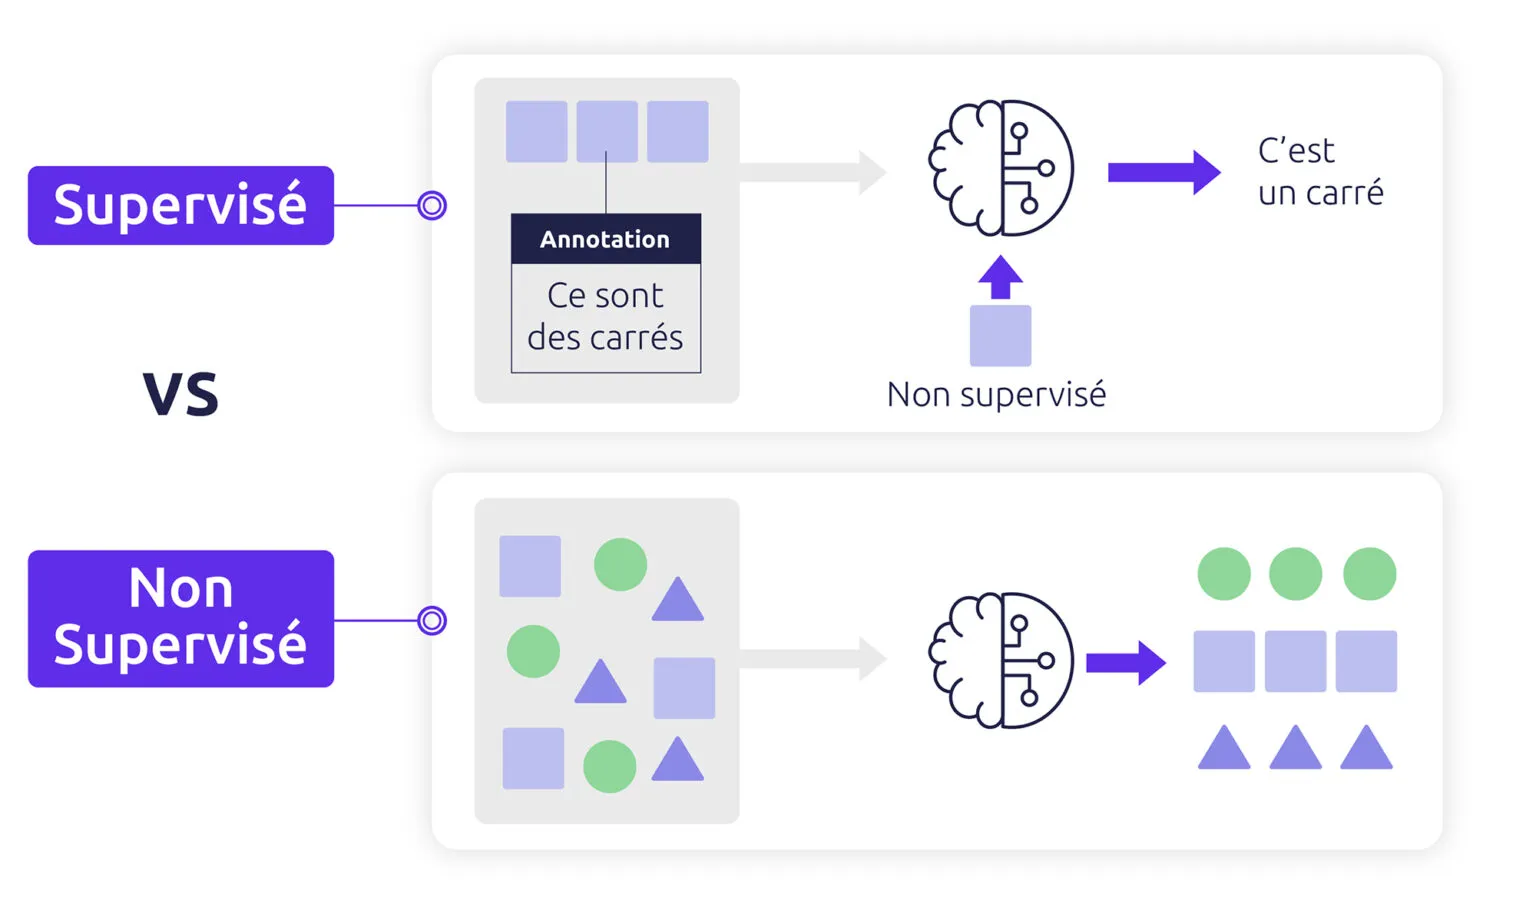
\includegraphics[width=0.7\textwidth,height=0.3\textheight]{img/non_supervisé_vs_supervisé.png}
     \caption{shéma montrant la différence majeur entre les algorithmes supervisés et non-supervisés \cite{non_supervisé_vs_supervisé}}
     \label{fig:example7}
     \end{figure}


\subsubsection{Apprentissage semi-supervisé(Semi-Supervised Learning) }
Dans cet apprentissage, toutes les données seraient structurées et étiquetées avant d'être placées dans un système. Mais comme ce n'est évidemment pas possible, l'apprentissage semi-supervisé constitue une solution envisageable lorsqu'on utilise de gros volumes de données brutes et non structurées. Ce type de modèle consiste à insérer de petites volumes de données étiquetées pour enrichir des ensembles de données non étiquetés. Un algorithme d'apprentissage semi-supervisé invite la machine à analyser les données étiquetées afin de déterminer des propriétés corrélatives qui pourraient être appliquées aux données non étiquetées.\cite{what_is_machine_learning}

\textbf{Applications des techniques d'apprentissage semi-supervisé \cite{what_is_machine_learning}:}
\begin{itemize}[label={*}]
\item L'analyse du discours et de la langue.
\item Les recherches médicales complexes.
\item Détection de fraude à un niveau général.
\item etc ...
\end{itemize}

\vspace{2cm}


\subsubsection{Apprentissage par renforcement (Reinforcement Learning)}
Il désigne l’ensemble des méthodes qui permettent à un agent(machine) d’apprendre à choisir quelle action prendre, et ceci de manière autonome .
Plongé dans un environnement donné, il apprend en recevant des récompenses ou des pénalités en fonction de ses actions. Au travers de son expérience, l’agent cherche à trouver la stratégie décisionnelle optimale qui puisse lui permettre de maximiser les récompenses accumulées au cours du temps.

     \begin{figure}[htbp]
     \centering    
     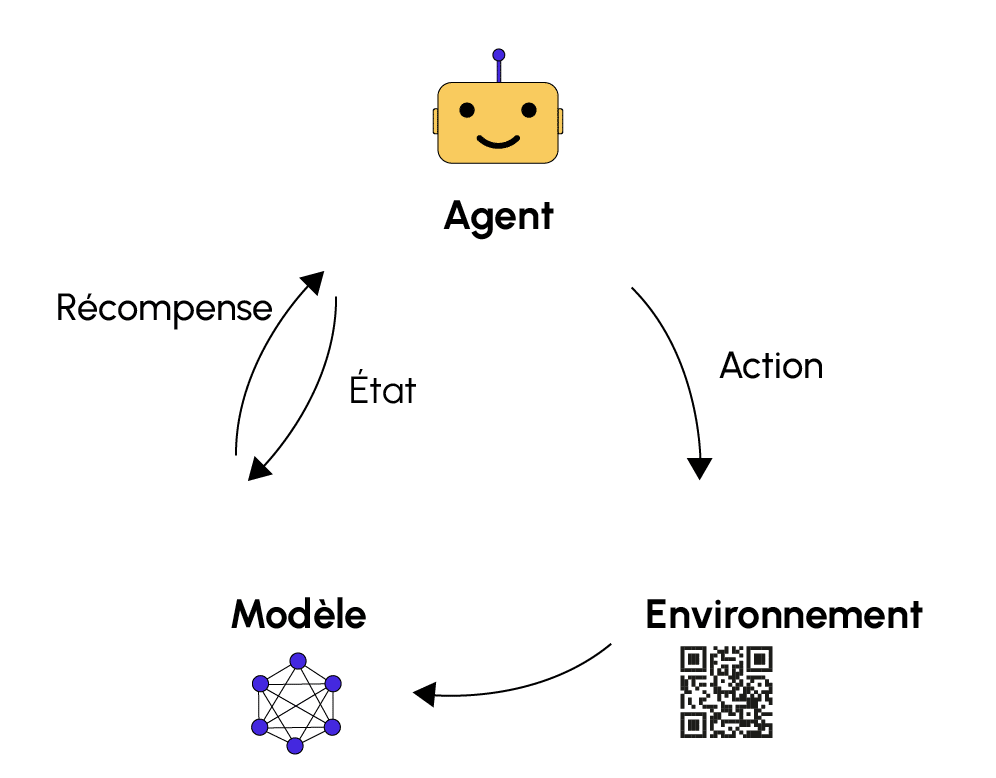
\includegraphics[width=0.7\textwidth,height=0.3\textheight]{img/reinforcement_learning.png}
     \caption{schéma résumant le processuss des algorithmes d'apprentissage par renforcement \cite{reinforcement_learning}}
     \label{fig:example8}
     \end{figure}

\vspace{1cm}     
\textbf{Techniques de l'apprentissage par renforcement :}
Il existe un certain nombre des méthodes les plus connues \cite{basics_of_reinforcement_learning} :
\begin{itemize}[label=$\bullet$]
\item \textbf{Q-learning} : un algorithme qui estime la valeur des paires état-action et met à jour de manière itérative les valeurs Q en fonction des récompenses observées. En apprenant une politique optimale directement à partir de l'expérience, Q-learning permet aux agents de prendre des décisions intelligentes
\item \textbf{Réseaux Q-profonds (DQN)} : Les réseaux Q profonds (DQN) combinent l'apprentissage par renforcement avec des réseaux de neurones profonds. Les DQN utilisent la puissance des architectures d'apprentissage profond pour se rapprocher des valeurs Q pour de grands espaces d'état-action. En utilisant des réseaux de neurones comme approximateurs de fonctions, les DQN peuvent gérer des environnements complexes et apprendre des représentations de grande dimension. Les DQN ont obtenu un succès remarquable dans différents domaines tels que jouer à des jeux Atari et contrôler des systèmes robotiques.
\item \textbf{Méthodes de gradients de politique} : Les méthodes de gradient de politique optimisent directement la politique en estimant les gradients des récompenses attendues par rapport aux paramètres de la politique. En mettant à jour de manière itérative la politique dans le sens de récompenses plus élevées, ces méthodes peuvent apprendre des politiques d’action complexes et continues. Les algorithmes de gradient de politique ont connu du succès dans des applications telles que le contrôle robotique et le traitement du langage naturel.
\item \textbf{Optimisation de la politique proximale (PPO)} : est un algorithme d'optimisation qui maintient un équilibre entre stabilité et efficacité des échantillons. PPO utilise une fonction d'objectif de substitution pour mettre à jour les paramètres de politique et garantir de petites mises à jour de politique afin de maintenir la stabilité. PPO a démontré des performances supérieures dans divers domaines tels que le jeu et la manipulation robotique.
\end{itemize}
\vspace{1cm}
Il existe d'autres méthodes qui ont été apparu avec l'avancement de ce type d'apprentissage , y compris l'apprentissage par renforcement multi-agents et le méta-apprentissage .

\textbf{Applications des techniques d'apprentissage par renforcement \cite{basics_of_reinforcement_learning}:}
\begin{itemize}[label={*}]
\item Robotique.
\item Véhicules autonomes.
\item Systèmes de recommandation.
\item etc ...
\end{itemize}


\newpage

\subsubsection{Différences entre les types d'apprentissage automatique} 
 \begin{figure}[htbp]
     \centering    
     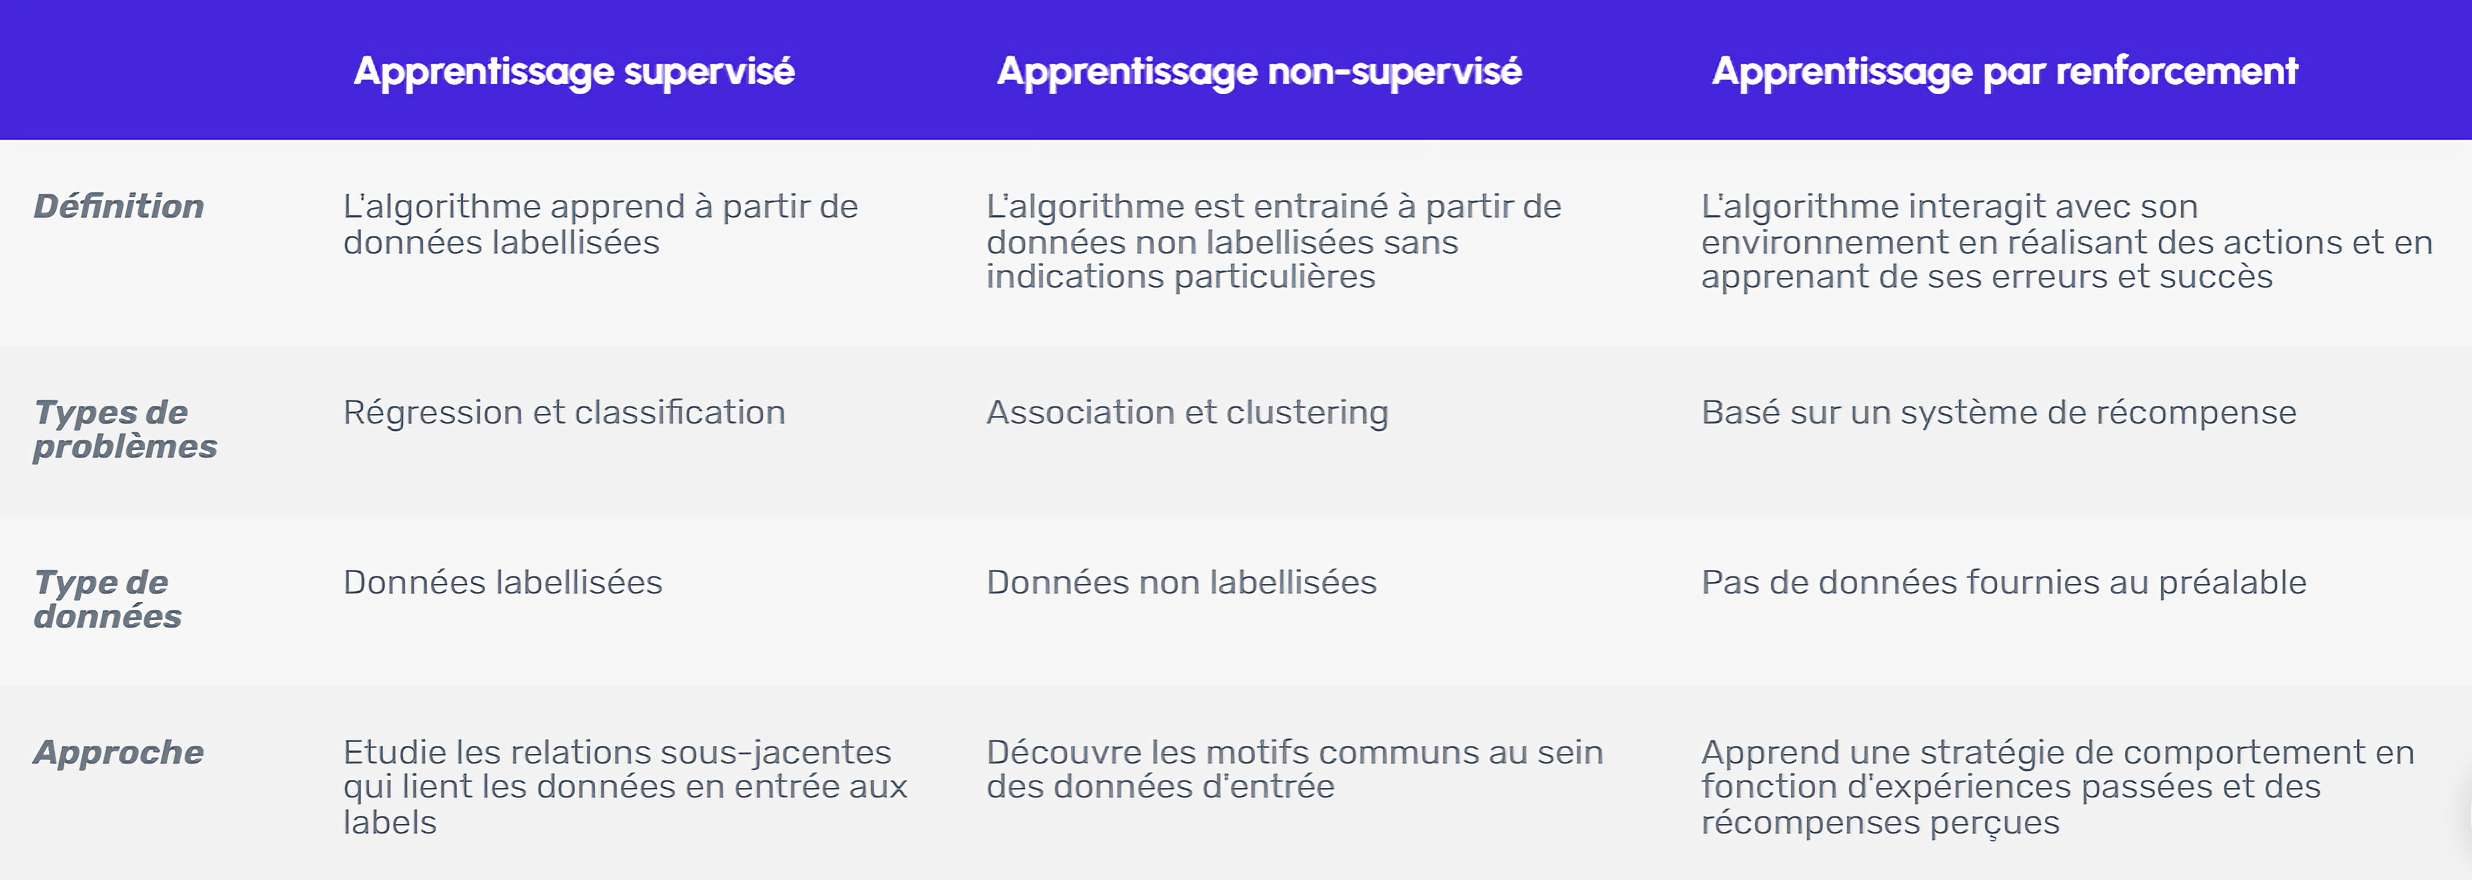
\includegraphics[width=1\textwidth,height=0.3\textheight]{différences.png}
     \caption{Différences entre les types d'apprentissage automatique \cite{reinforcement_learning}}
     \label{fig:example9}
     \end{figure}

 \vspace{3cm}    
 \section{Apprentissage profond}
  Le deep learning (Apprentissage profond) est une façon particulière de faire du machine learning (le deep learning(DL) est un sous-ensemble de techniques du machine learning), il se focalise sur des méthodes d'apprentissage automatique qui s'inspirent du fonctionnement du système nerveux de l'être humain.
 
 Contrairement à l'apprentissage automatique qui comprend des algorithmes de réseaux de neurones simples(nous allons clarifier cette notion après) , le deep learning comprend des techniques de réseaux de neurones avec des architectures beaucoup plus complexe (les notions "complexe" , "simple" et "couches" dans Table 1.1 vont être clarifiées après) .
 

\begin{center}
\begin{table}[htbp]
\begin{tabular}{|p{8cm}|p{8cm}|}
\hline
\textbf{NN du machine learning} & \textbf{NN du deep learning} \\ \hline
\hline
- Architecture simple (1-2 couches cachées) & - Architecture complexe (plusieurs couches cachées qui peuvent atteindre les centaines) \\
\hline
- Moins de puissance de calcul & - puissance de calcul trop importante \\
\hline
- Apprentissage souvent supervisé & - Apprentissage supervisé, non supervisé ou par renforcement \\
\hline
- Besoin d'une intervention humaine pour l'extraction des caractéristiques & - Pas besoin d'une intervention humaine \\
\hline
- traitement et observation des milliers de données & - traitement et observation d'une grande massivité de données (Big data)\\
\hline
- Applications: systèmes de recommandation , classification d'images, reconnaissance faciale, détection de fraude & - Applications: les applications du machine learning ,traitement du langage naturel, vision par ordinateur, traduction automatique \\
\hline
- utilisé par le data Analyst et data scientist & - utilisé par le data scientist seulement\\
\hline
\end{tabular}
\caption{Differences entre les réseaux de neurones du ML et du DL}
\end{table}
\end{center}


 \subsubsection{Principe des NN profonds}
 Ces algorithmes sont composés d'unités reliées entre elles qui vont s'entre activer (comme le cerveau humain) qu'on les appelle "neurones artificiels" , chaque neurone du réseau peut produire un effet sur ceux auxquels il est connecté. Ce qui presque commun entre toutes ces réseaux est que ces neurones sont organisés sous forme de couches (une couche d'entrée qui contient les neurones représentant les variables d'entrée , une couche de sortie qui contient le/les neurone(s) de sortie , et un certain nombre de couches cachées) reliées entre eux par la liaison entre le neurones des différentes couches . Toutefois, au lieu d'un signal électrique (comme dans le cerveau humain), le réseau de neurones attribue un certain poids à différents neurones .
    
    \begin{figure}[htbp]
     \centering  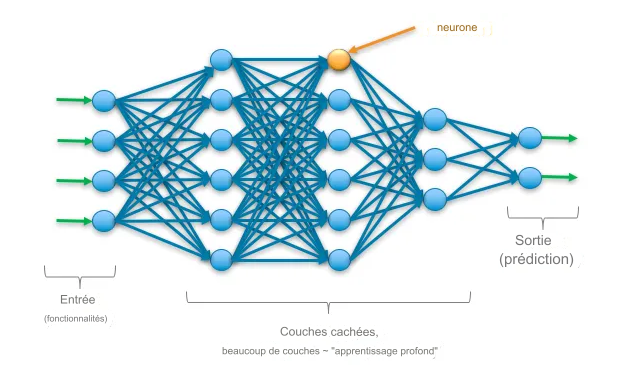
\includegraphics[width=0.8\textwidth,height=0.3\textheight]{img/NN.png}
     \caption{schéma d'un réseau de neurones profond (avec 3 couches cachées) }
     \label{fig:example10}
     \end{figure}
 \newpage
 
 \textbf{Modèles des réseaux de neurons profonds :} 
On ne peut jamais déterminer le nombre des architectures des NN créées jusqu'aujourd'hui (voir par exemple la figure~\ref{fig:NN_architectures} pour un aperçu des architectures de réseaux neuronaux.) , parce c'est une ensemble de modèles qui dépendent à plusieurs facteurs (prenons l'exemple des architectures citées dans la figure 1.10) , il suffit d'effectuer un petit changement dans un seul de ces facteurs et on va avoir un nouveau modèle . Parlant des facteurs , nous citons :

    \begin{itemize}[label=$\bullet$]
    \item \textbf{Architecture : }La topologie peut se différer beaucoup entre les architecture , dépandant des liasions entre les neurones quelque soit leurs couches ( comme c'est le cas dans les architectures citées dans la figure 1.10))
    
    \item \textbf{Taille du réseau :} Le nombre de neurones dans chaque couche peut être différent d'une couche à l'autre , sans parler de la différence de ce nombre entre les différentes architecture.
 
    \item \textbf{La profondeur du réseau :} nous pouvons avoir une architecture avec 3 couches cachées comme on peut trouver une architecture avec de centaines de couches cachées
    
    \item \textbf{Fonctions d’activation :} la fonction d'activation est une fonction mathématique appliquée à un signal en sortie d'un neurone artificiel . Elle va permettre le passage ou non de l’information si le seuil de stimulation est atteint. Concrètement, elle va avoir pour rôle de décider si on active ou non une réponse du neurone.
    Dans la figure 1.10 se mentionne les fonctions d'activation les plus connues , mais il y on a d'autres comme c'est plus détaillé dans \cite{nwankpa2018activation}
    
    \begin{figure}[htbp]
     \centering    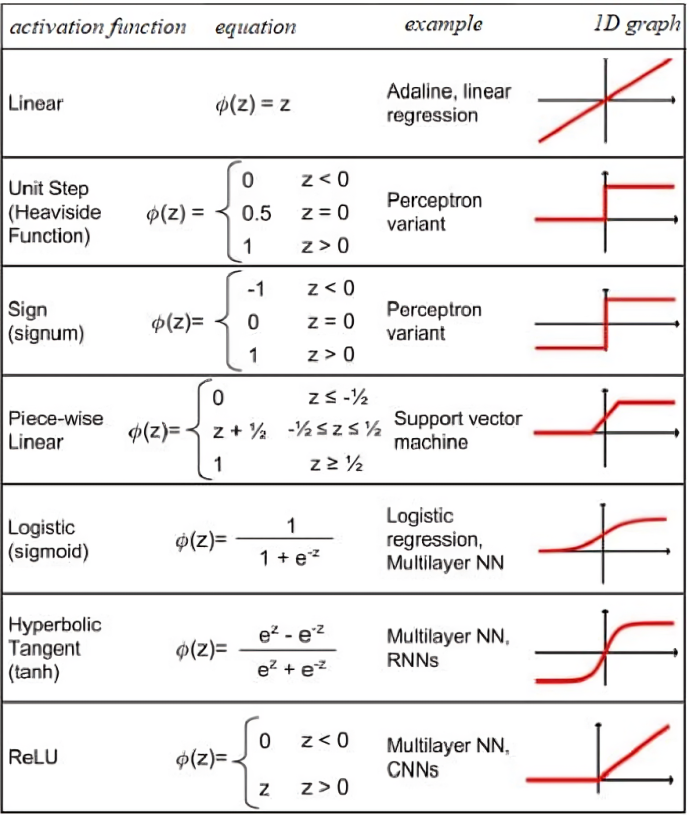
\includegraphics[width=0.65\textwidth,height=0.35\textheight]{activation_functions2.png}
     \caption{fonctions d'activtion dans un algorithme de NN profond\cite{activation_functions} }
     \label{fig:example11}
     \end{figure}
     \newpage
    \item \textbf{La pondération des connexions entre les neurones :} chaque connexion entre 2 neurones artificiels est pondérée par une valeur négative ou positive contrôlant l'impact des données communiquées entre ces unités . 
    \item \textbf{Valeur du biais:} c'est une valeur constante (ou un vecteur constant) ajoutée au produit des entrées et des poids dans un neurone artificiel afin d'affecter la sortie de la fonction d'activation.
    
    \begin{figure}[htbp]
     \centering  
     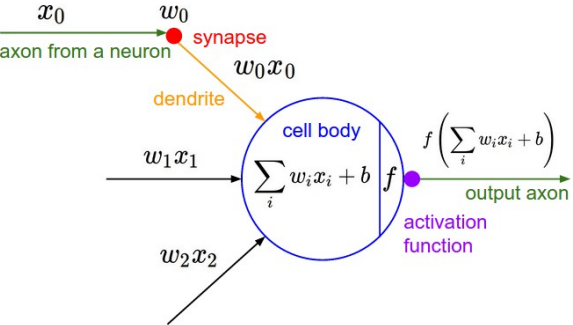
\includegraphics[width=0.55\textwidth,height=0.2\textheight]{neurone_detail.png}
     \caption{Schéma des opérations dans et entre les neurones artificiels\cite{neurone_detail} }
     \label{fig:example12}
     \end{figure}
    
    \item \textbf{Type de régularisation:}la régularisation comprend un ensemble de technique pour éviter le surapprentissage (overfitting) y compris :  \textbf{Normalisation ,dropout, régularisation L1 et L2 , et Early Stopping} 
    
    \item \textbf{Type de rétropropagation:} la rétropropagation est un ensemble de technique utilisées pour ajuster les poids des connexions entre les neurones , y compris \textbf{Rétropropagation avec Momentum , avec AdaGrad , avec Nesterov  gradient acceleré ,avec RMSProp , avec Adam , etc ... }
    
    \end{itemize}
    
    
   %  \begin{figure}
   %  \centering    
   %  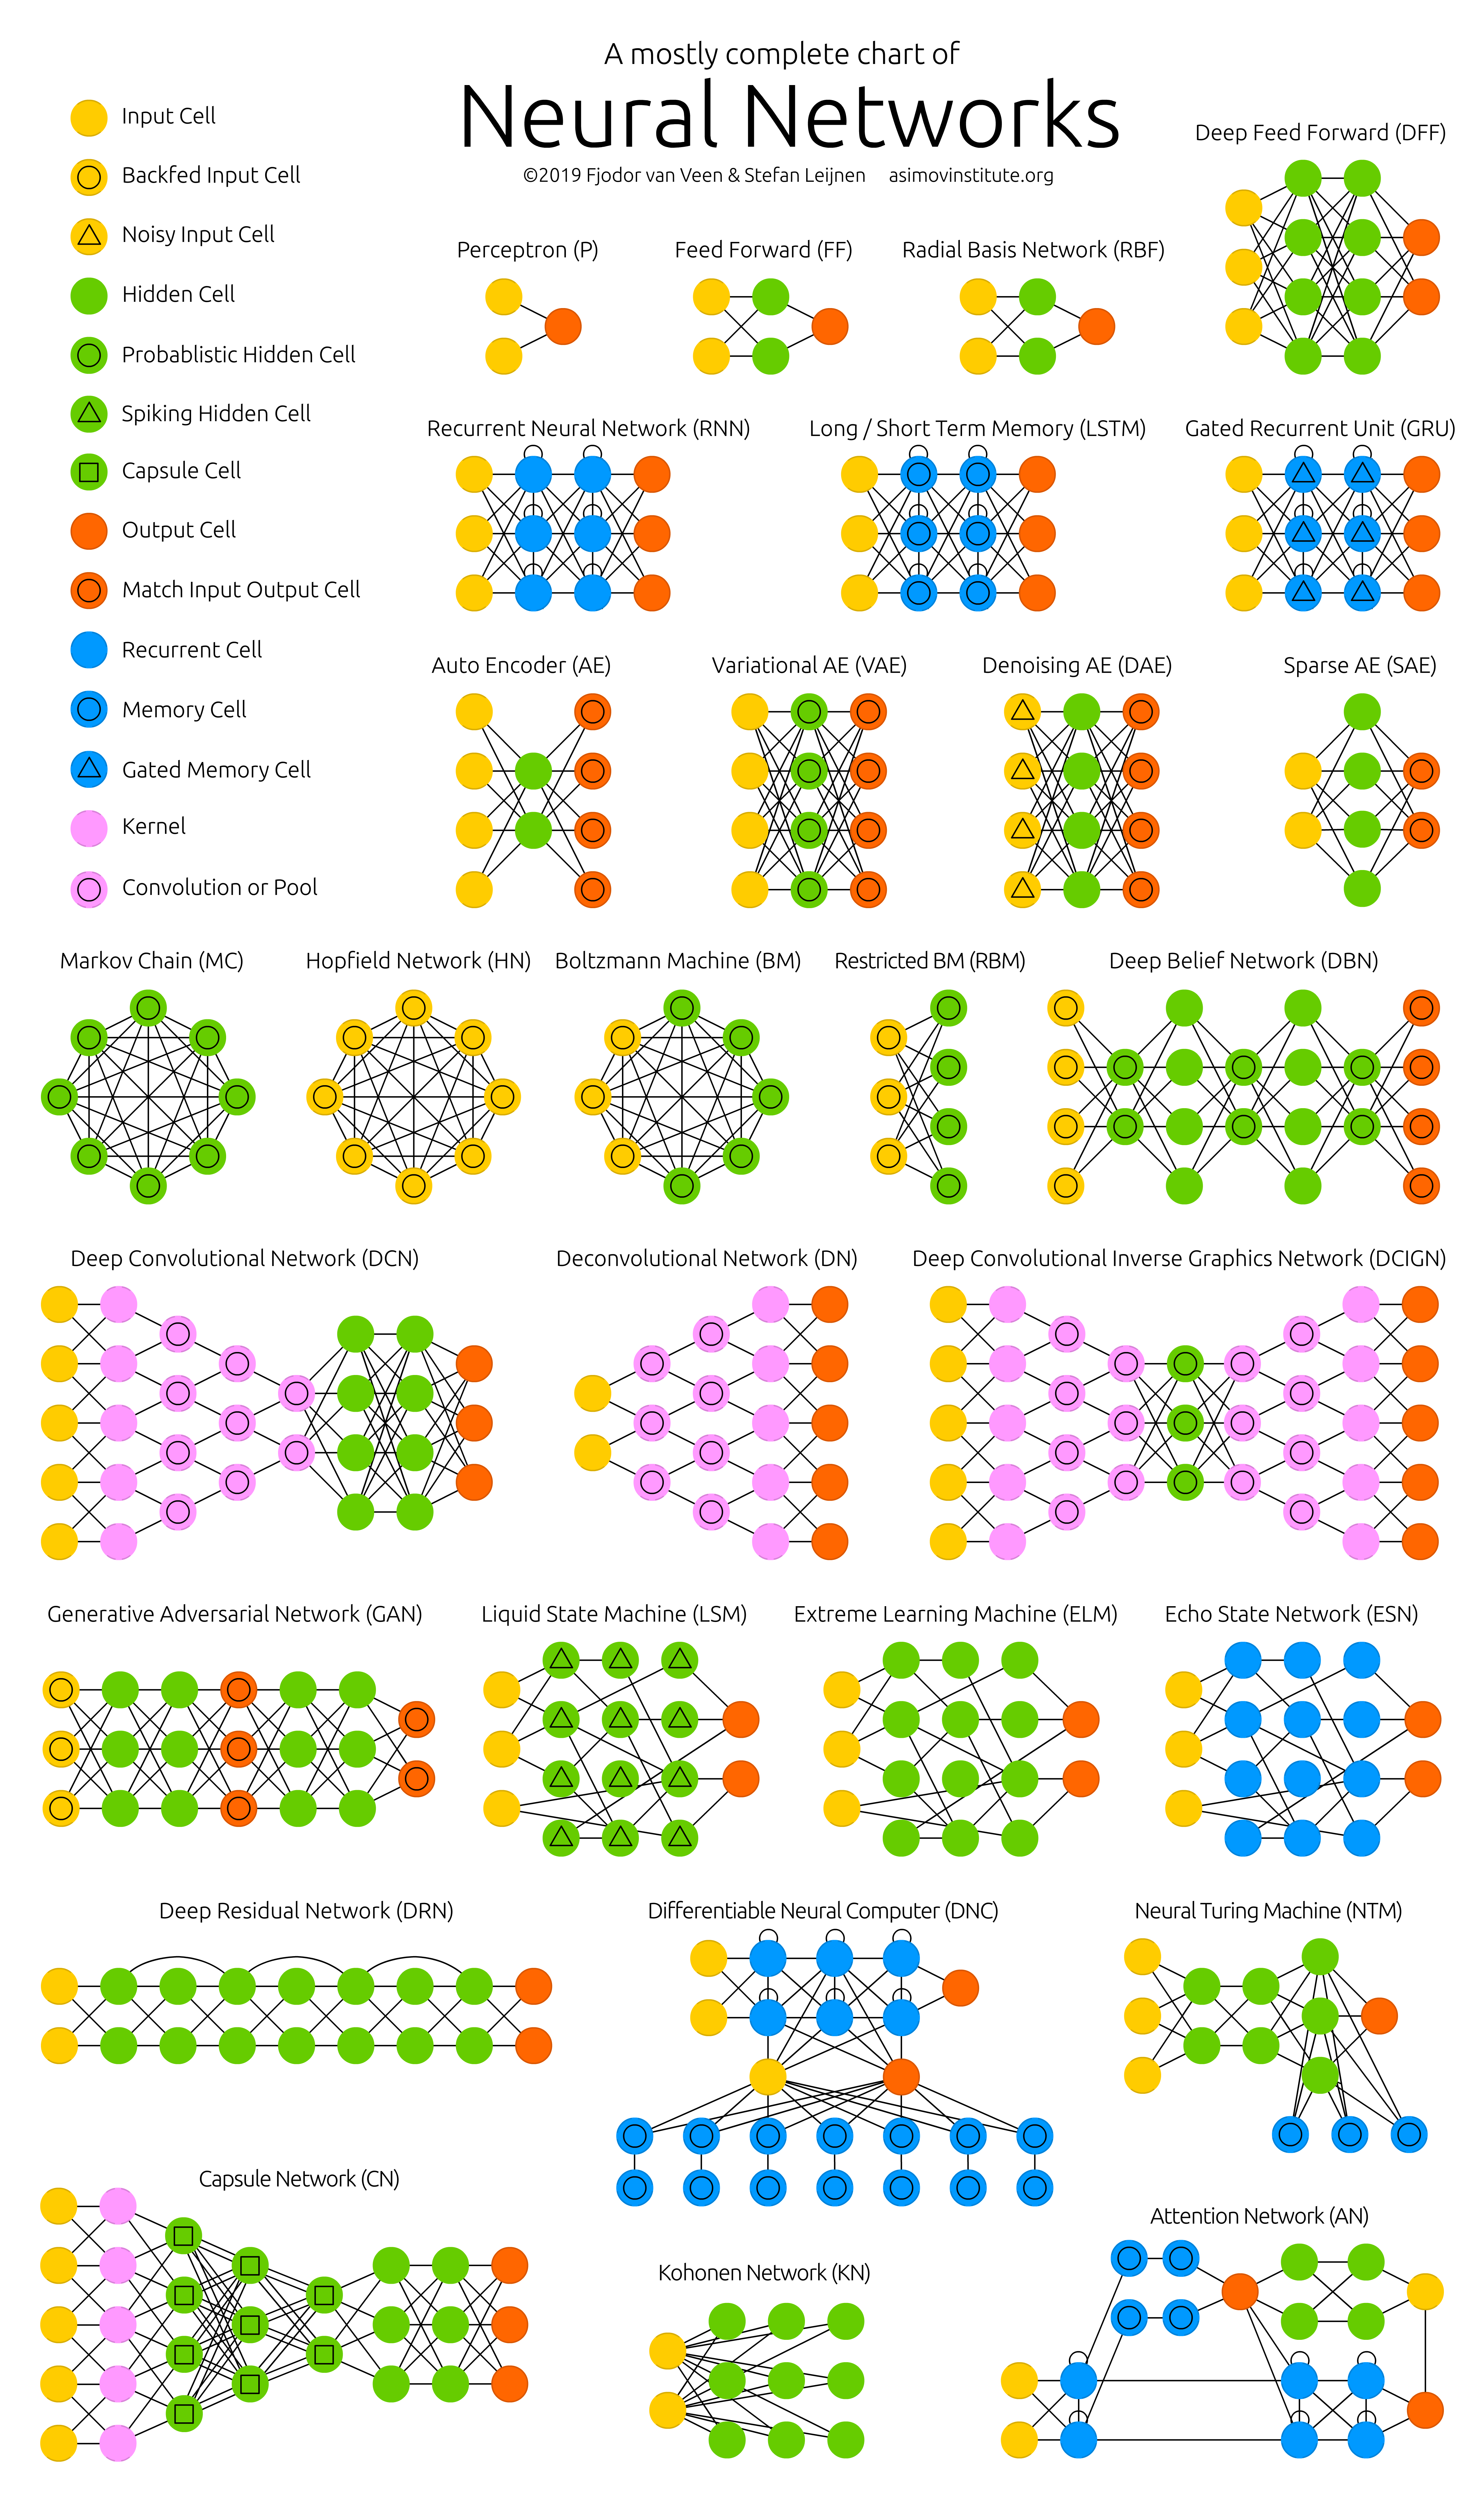
\includegraphics[width=1\textwidth,height=0.95\textheight]{NeuralNetworkZo19High.png}
   %  \caption{Un aperçu des architectures de réseaux neuronaux\cite{leijnen2020neural}}
   %  \label{fig:example13}
   %  \end{figure}



 \subsubsection{Types d'algorithmes d'apprentissage pronfond}
 Il existe différents types d'algorithmes , tel que \cite{algorithmes_deep_learning} :
 \begin{itemize}[label=$\bullet$]
\item \textbf{Réseaux neuronaux convolutifs (CNN) :}
les CNN (appelés aussi ConvNets) sont constitués d'une multitude de couches chargées de traiter et d'extraire les caractéristiques des données. De manière spécifique, les CNNs sont utilisés pour l'analyse et la détection d'objets.Donc , Ils peuvent donc servir dans le domaine vision ppar ordinateur (reconnaître des images satellites, traiter des images médicales, détecter des anomalies ou prédire des séries chronologiques, etc ...)

    \begin{figure}[htbp]
    \centering
    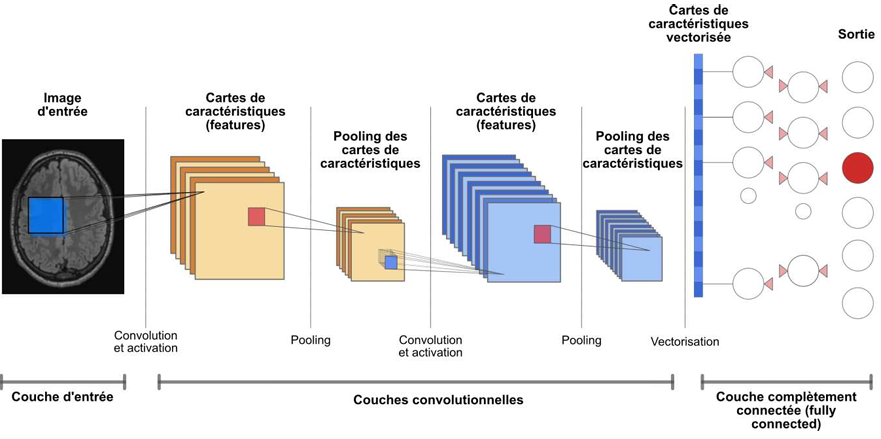
\includegraphics[width=0.6\textwidth,height=0.3\textheight]{CNN.png}
    \caption{Schéma général de principe de fonctionnement d'un réseau de neurones convolutifs \cite{fernandez_maloigne2019}.}
    \label{fig:example14}
    \end{figure}

\item \textbf{Réseaux neuronaux récurrents (RNN) :}
Les RNNs possèdent des connexions qui constituent des cycles dirigés. Cela permet aux sorties du LSTM (que nous allons le mentionner après) d'être exploitées comme entrées au niveau de la phase actuelle. Elle peut donc mémoriser les entrées précédentes à l'aide de sa mémoire interne. Dans la pratique, les RNN sont utilisés pour le sous-titrage d'images, le traitement du langage naturel et la traduction automatique.

    \begin{figure}[htbp]
    \centering
    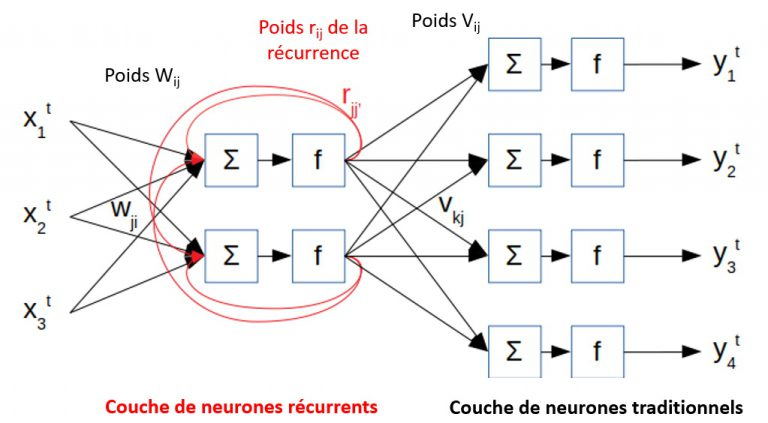
\includegraphics[width=0.4\textwidth,height=0.2\textheight]{RNN.jpg}
    \caption{Couche de neurones récurrents devant une couche de neurones traditionnels.
    \cite{LSTM}}
    \label{fig:example15}
     \end{figure}
     \newpage

 
\item \textbf{Réseaux de mémoire à long et court terme (LSTM) :}Les LSTM sont des dérivés de RNN. Ils peuvent apprendre et mémoriser des dépendances sur une longue durée. Les LSTM conservent ainsi les informations mémorisées sur le long terme. Ils sont particulièrement utiles pour prédire des séries chronologiques, car ils se rappellent des entrées précédentes. Outre ce cas d'utilisation, les LSTM sont également utilisés pour composer des notes de musique et reconnaître des voix.

    \begin{figure}[htbp]
    \centering
    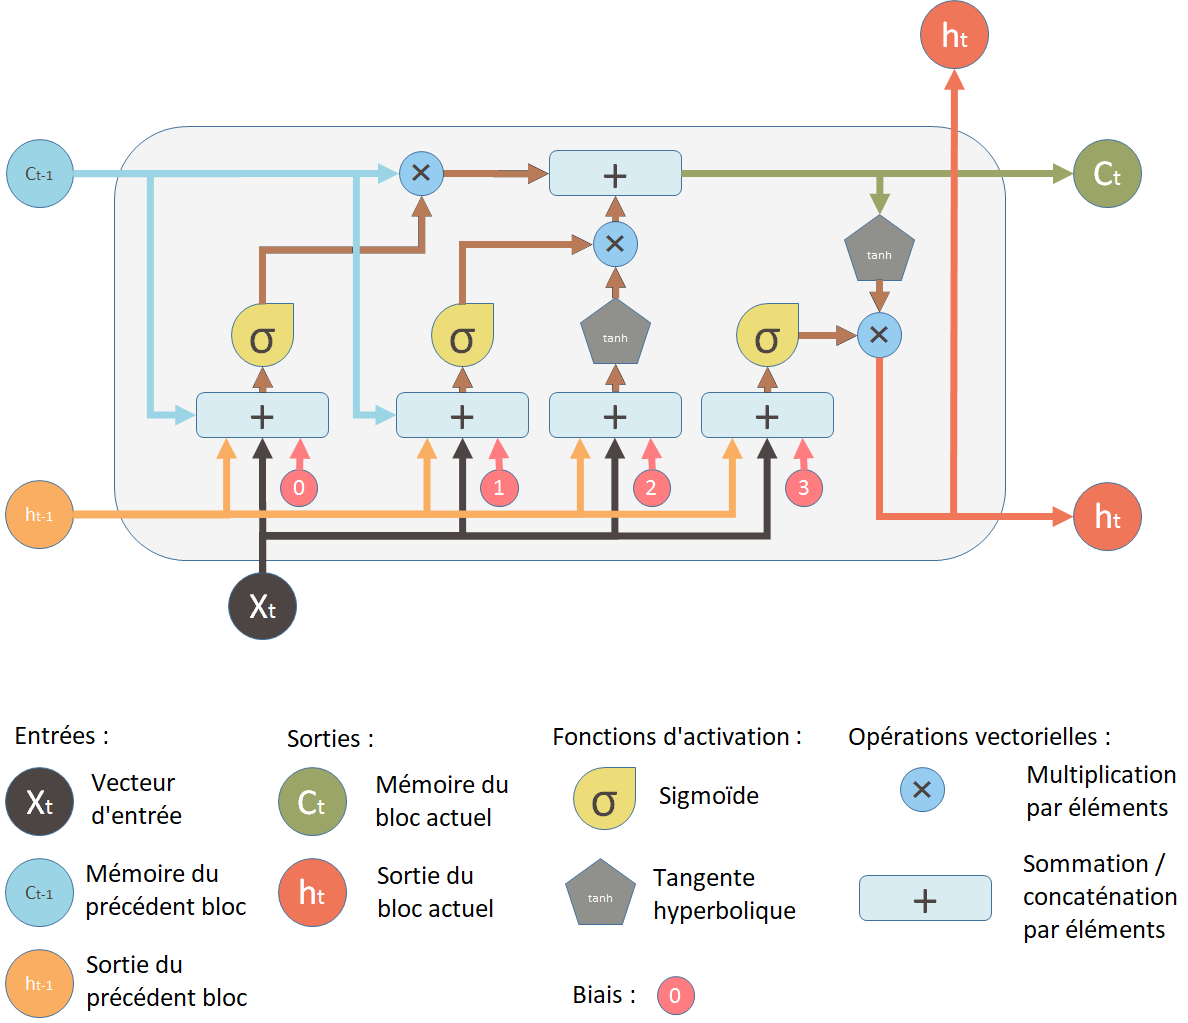
\includegraphics[width=0.6\textwidth,height=0.3\textheight]{img/LSTM.png}
    \caption{Schéma d'un exemple de réseau LSTM.
    \cite{LSTM}}
    \label{fig:example16}
    \end{figure}
     
\item \textbf{Réseaux adversariaux génératifs (GAN) :}
Les GAN créent de nouvelles instances de données qui s'apparentent aux données d'apprentissage profond. Ils possèdent deux principaux composants : un générateur et un discriminateur. Si le générateur apprend à produire des informations erronées, le discriminateur, quant à lui, apprend à exploiter ces fausses informations. Les GAN sont généralement utilisés par les créateurs de jeux vidéo pour améliorer les textures 2D.

    \begin{figure}[htbp]
    \centering
    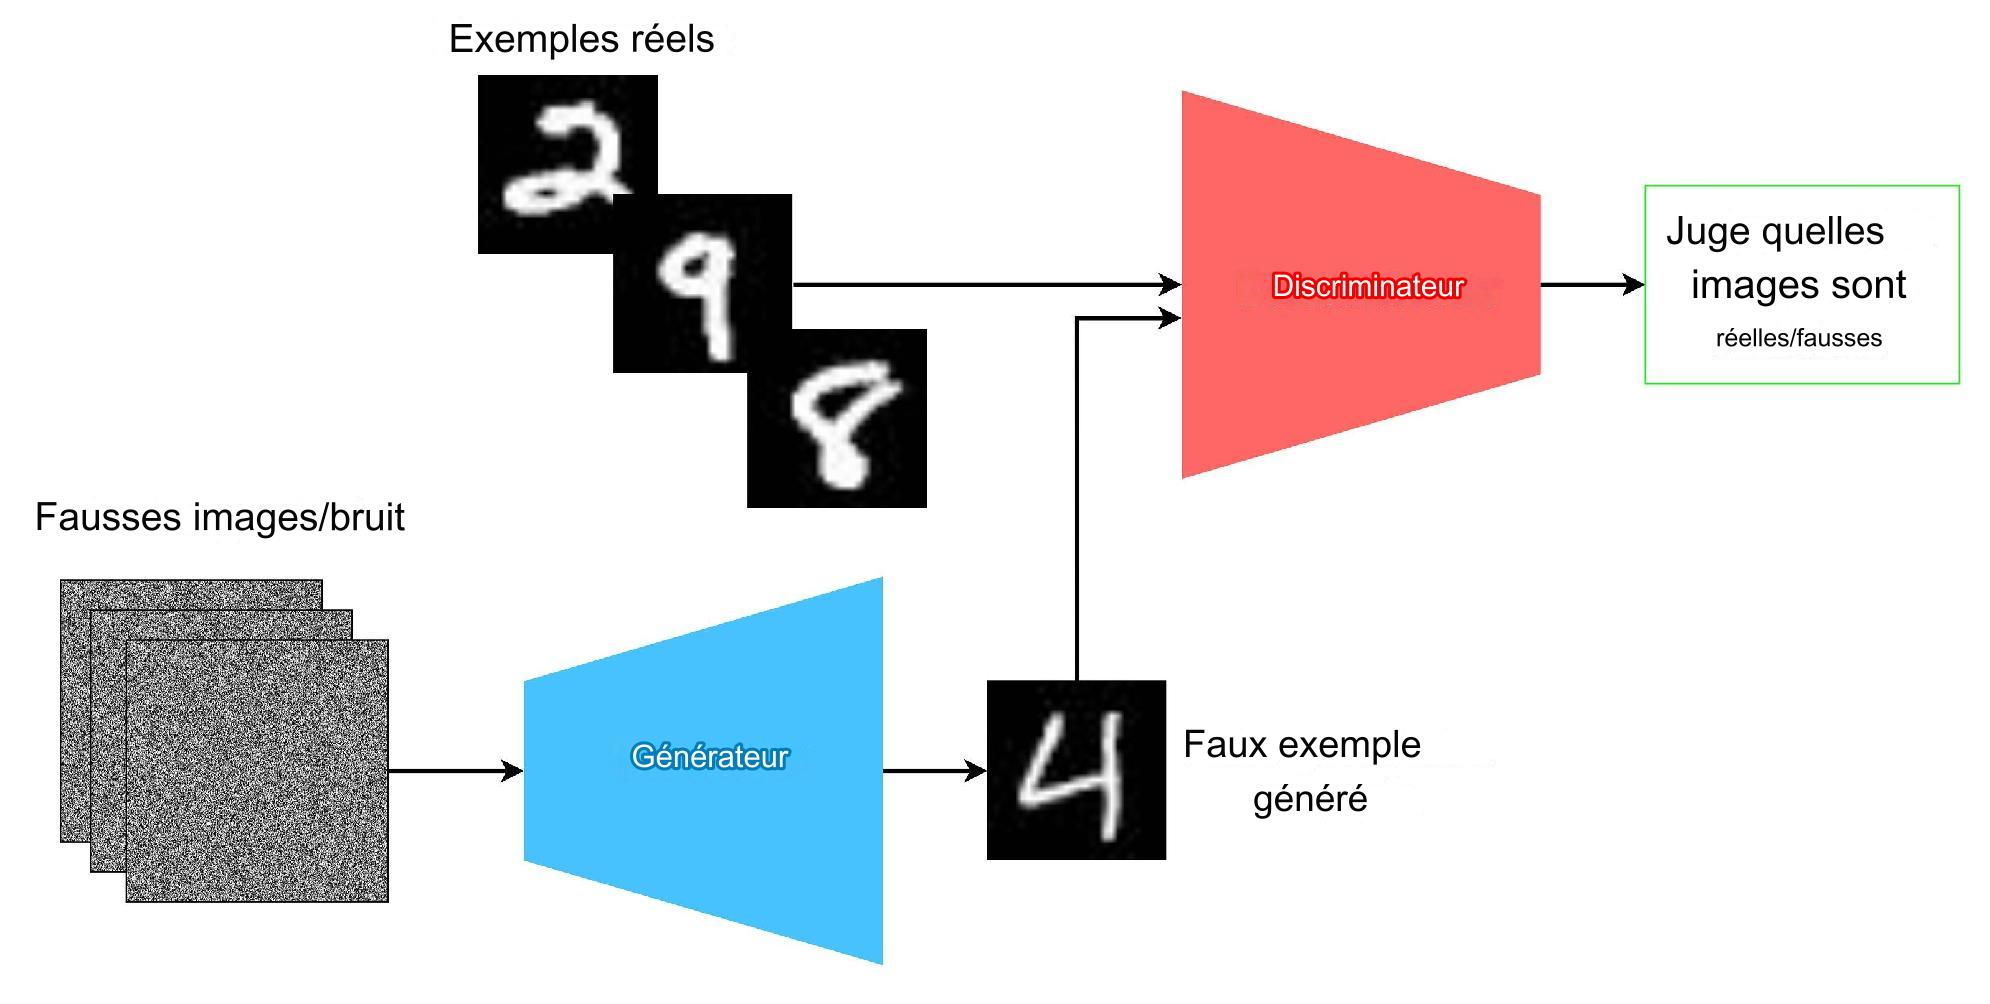
\includegraphics[width=0.9\textwidth,height=0.3\textheight]{img/GAN.jpg}
    \caption{Schéma decriptif du principe des GANs.
    \cite{generative_adversarial_networks_explained/}}
    \label{fig:example17}
    \end{figure}

\item \textbf{Machines de Boltzmann restreintes (RBM) :}
Ce sont des réseaux neuronaux stochastiques(avec des probabilités) constitués de deux couches : unités visibles et unités cachées. Ces réseaux artificiels sont capables d'apprendre en partant d'une distribution de probabilité sur un ensemble d'entrées. 
    
    \begin{figure}[htbp]
    \centering
    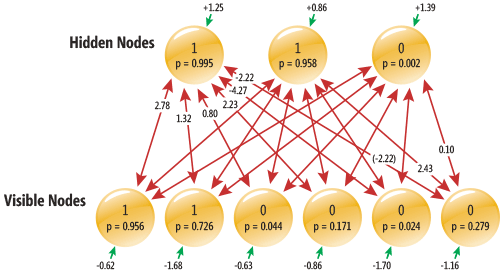
\includegraphics[width=0.6\textwidth,height=0.2\textheight]{img/RBM.png}
    \caption{Schéma d'un exemple de machines de Boltzmann restreintes.
    \cite{RBM}}
    \label{fig:example18}
    \end{figure}

Néanmoins, il est important de souligner que la liste d'algorithmes présentés ci-dessus n'est pas exhaustive. Il en existe d'autres types comme :
- les auto-encodeurs,
- les réseaux de croyance profonds (DBN),
les perceptrons multicouches (MLP).
- Les cartes auto-organisées (SOM) 
\end{itemize}


     
\subsection{Apprentisssage ensembliste}
Aussi appelé ensemble learning, c'est un ensemble de techniques qui combinent plusieurs algorithmes d’apprentissage automatique pour améliorer la précision des prédictions que celles obtenues avec un de ces algorithmes .

\subsubsection{Types des techniques d'apprentissage ensembliste} 
\begin{itemize}[label=$\bullet$] 

\item \textbf{Bagging (Bootstrap Aggregating)} :
Il consiste à entraîner plusieurs modèles ( du même type généralement ) sur des sous-ensembles aléatoires du jeu de données d’entraînement.
Chaque modèle est formé indépendamment, ce qui va réduir la variance et le surajustement (overfitting).
Les prédictions de ces modèles sont par la suite agrégées par vote majoritaire ou moyenne pour obtenir une prédiction finale plus robuste.
L’exemple le plus célèbre de bagging est l’algorithme Random Forest.

\item \textbf{Boosting} :
C'est un ensemble de modèles relativement faibles en séquence.
Chaque modèle est ajusté pour corriger les erreurs du modèle précédent. Les observations mal prédites (par les modèles précédents) reçoivent plus de poids, ce qui permet d’améliorer progressivement la performance globale.
Parmi les exemples populaires de boosting on trouve : \\ \textbf{AdaBoost} : Il ajuste de manière itérative le poids des observations en accordant plus d’importance à celles qui sont mal classées afin d'avoir un modèle fort qui est une combinaison de modèles relativement faibles .) \\
\textbf{Gradient Boosting} : Il optimise une fonction de perte en utilisant des gradients pour ajuster les prédictions du modèle.
Le gradient boosting est largement utilisé dans les compétitions de machine learning..

    \begin{figure}[htbp]
     \centering    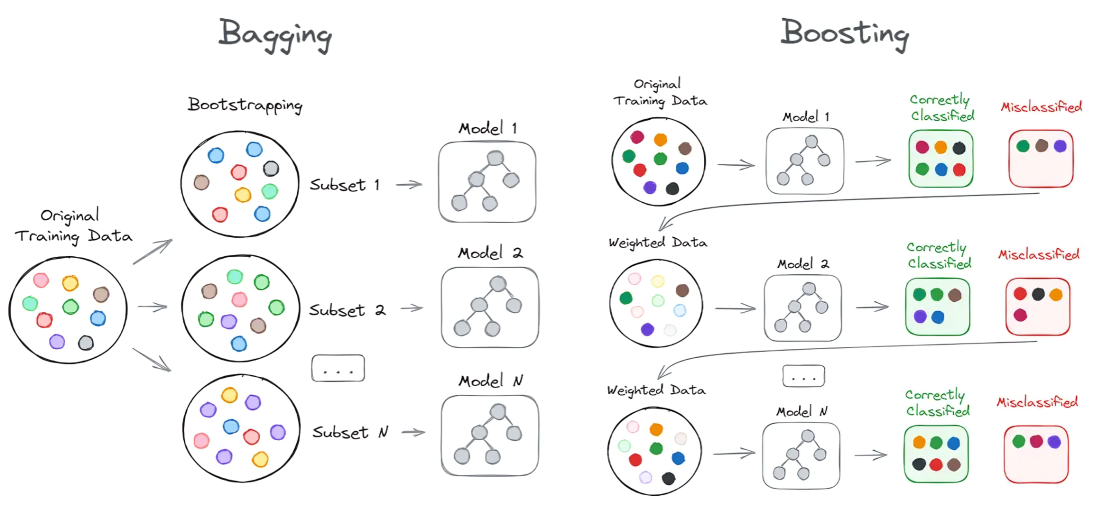
\includegraphics[width=0.7\textwidth,height=0.22\textheight]{img/baggingVSboosting.png}
     \caption{Schéma montrant la différence entre le bagging et le boosting \cite{sundararajan2021}}
     \label{fig:example19}
     \end{figure}
\item \textbf{Stacking} :
Le stacking (empilement) combine les prédictions de plusieurs modèles de base( après générer des prédictions sur les mêmes données d’entraînement.)
Par la suite, un modèle de méta-apprentissage (modèle de niveau supérieur) est utilisé pour combiner ces prédictions de manière optimale.
L'empilement permet d’exploiter les forces de différents types de modèles.

    \begin{figure}[htbp]
    \centering
    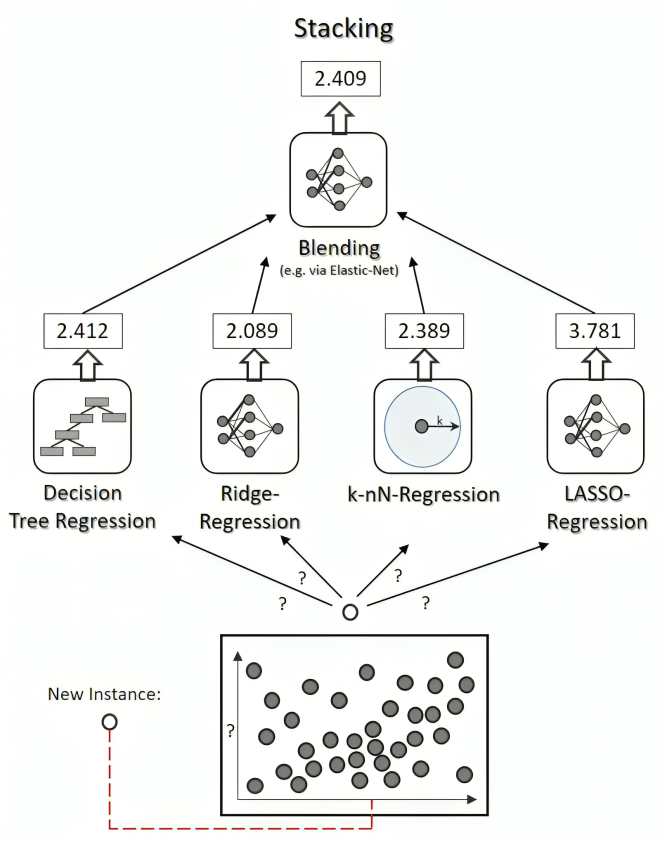
\includegraphics[width=0.55\textwidth,height=0.4\textheight]{stacking.png}
     \caption{Schéma d'un exemple du stacking\cite{stacking}}
     \label{fig:example20}
     \end{figure}
\newpage     
\item \textbf{Random Forest} :
Les forêts aléatoires sont des ensembles d’arbres de décision ,
chaque arbre est construit sur un sous-ensemble aléatoire du jeu de données . Les prédictions de chaque arbre sont agrégées par vote majoritaire, le truc qui va réduire l'overfitting et améliore la généralisation.

\begin{figure}[htbp]
     \centering    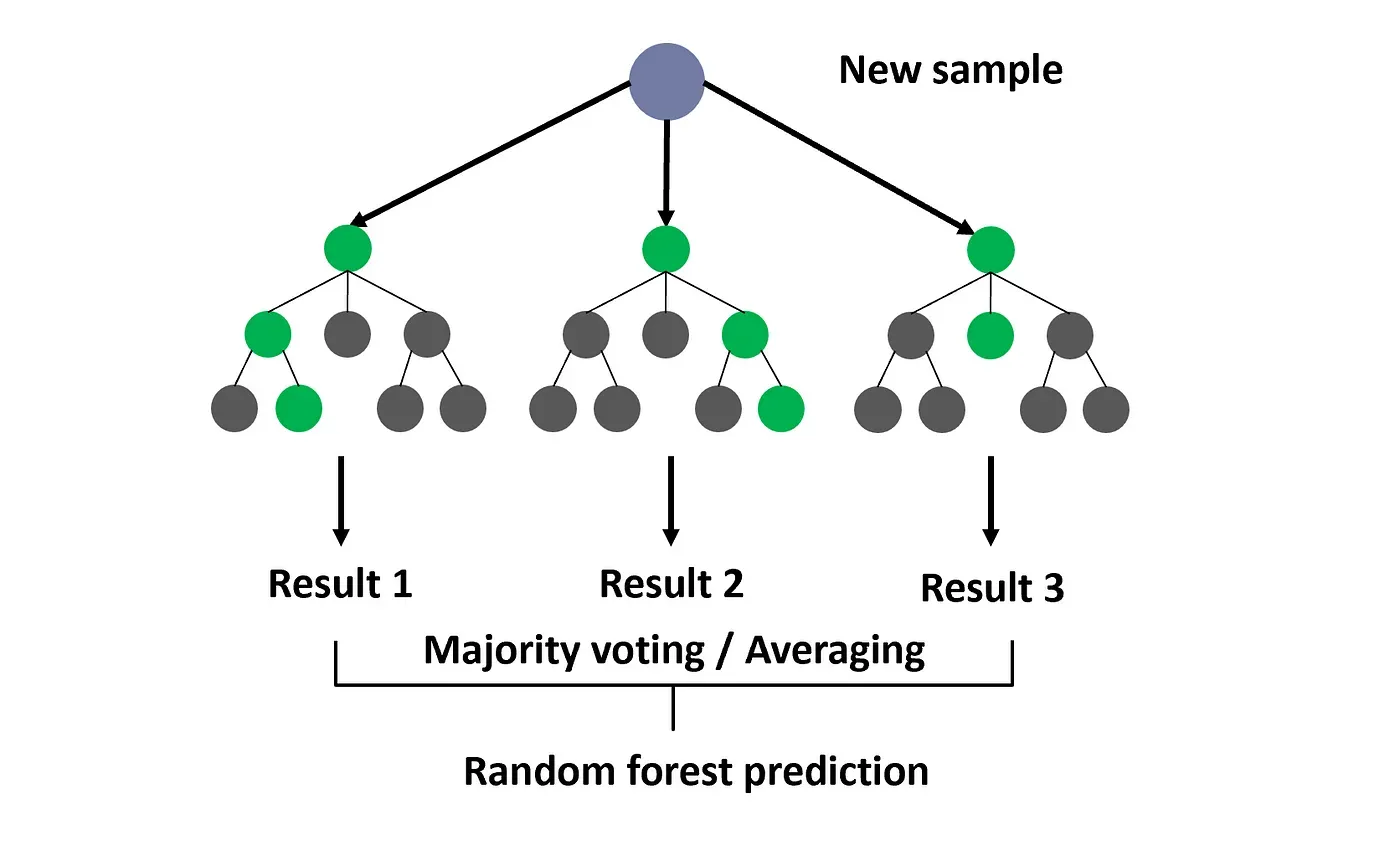
\includegraphics[width=0.6\textwidth,height=0.3\textheight]{img/random_forest.png}
     \caption{Schéma exemplaire d'une architecture d'ensembl learning de random forest \cite{random_forest}}
     \label{fig:example21}
     \end{figure}



\end{itemize}
% \subsection{Modèle CNN_différentes couches}
\subsection{Apprentissage basé transfert}
Connu aussi par "transfert learning" , c'est une famille de technique d’apprentissage automatique qui profite des connaissances acquises lors de la résolution d’un problème (donc on a un modèle existant déja entrainé qui nous a aidé à acquéir des connaissances prêtes) pour les appliquer à un problème similaire ou plus spécifique.


\subsubsection{Types de techniques de transfert learning}
\begin{itemize}[label=$\bullet$] 

\item \textbf{Transfert proche (inductif)} : Il se produit à l’intérieur d’un même domaine de connaissance ou d’une discipline spécifique
Exemple : utiliser un modèle pré-entraîné pour la classification d'images pour une nouvelle tâche de classification d'images.

\item \textbf{Transfert lointain (transductif)} : Il se produit entre des domaines très différents et c'est plus général où la tâche cible et la tâche source sont différentes concernant la distribution de données, mais partagent des similarités structurelles.
Exemple : utiliser un modèle pré-entraîné pour la reconnaissance d'objets pour une nouvelle tâche de détection d'anomalies.

\end{itemize}



\subsection{Mesures d'évaluation des modèles}
L’évaluation des modèles d’apprentissage automatique profond est nécessaire pour savoir leurs performances et leurs précision à résulter la bonne prédiction. Alors,  nous utilisons des mesures quantitatives  qui fournissent un aperçu des performances du modèle et aident à comparer différents modèles ou algorithmes. On cite par exemple \cite{important_model_evaluation_error_metrics} \cite{classification_metrics_matrice_de_confusion} \cite{confusion_matrix_accuracy_recall_precision_false_positive_rate_and_f_scores_explained}:
\begin{itemize}[label=$\bullet$] 
\item \textbf{Matrice de confusion} : Elle résume les prédictions du modèle sur lequel s’appuient toutes les métriques de classification que nous allons citer : accuracy, F1-score, courbe ROC, Précision , Rappel ...etc en determinant les vrais positifs, les vrais négatifs, les faux positifs et les faux négatifs tels que :\\
\textbf{Vrai positif(TP)} : vous aviez prédit du positif, et c’est vrai.\\
\textbf{Vrai négatif(TN)} : vous avez prédit un résultat négatif, et c'est vrai.\\
\textbf{Faux positif(FP)(Erreur de type 1)} : vous avez prédit un résultat positif et c'est faux, en réalité c'est négatif.\\
\textbf{Faux négatif(FN)(Erreur de type 2)} : vous avez prédit un résultat négatif et c'est faux, en réalité c'est positif.\\
    \begin{figure}[htbp]
    \centering
    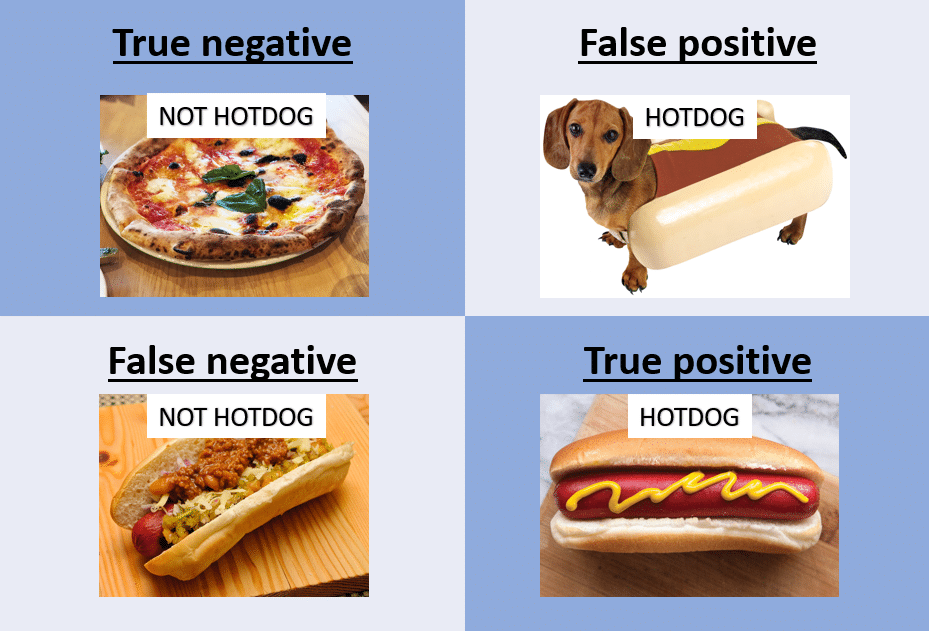
\includegraphics[width=0.5\textwidth,height=0.25\textheight]{matrice_confusion_elements.png}
    \caption{Illustration des éléments du matrice de confusion par images\cite{confusion_matrix_accuracy_recall_precision_false_positive_rate_and_f_scores_explained}}
    \label{fig:example22}
    \end{figure}
\item \textbf{Précision (Accuracy)} : Elle mesure le taux de prédictions correctes par rapport au nombre total d’échantillons positives .
\begin{equation}
\text{Precision} = \frac{\text{TP}}{\text{TP} + \text{FP}}
\end{equation}
\item \textbf{Rappel (Recall)} : Il évalue la capacité du modèle à détecter tous les exemples positifs. Donc , il correspond au taux d’individus positifs détectés par le modèle.
\begin{equation}
\text{Rappel} = \frac{\text{TP}}{\text{TP} + \text{FN}}
\end{equation}
    \begin{figure}[htbp]
    \centering
    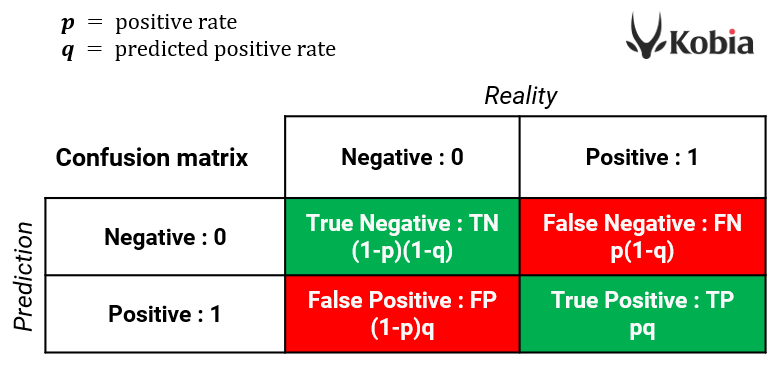
\includegraphics[width=0.7\textwidth,height=0.3\textheight]{calculs.png}
    \caption{Calculs des éléments du matrice de confusion\cite{classification_metrics_matrice_de_confusion}}
    \label{fig:example23}
    \end{figure}
\begin{align*}
p &= \frac{\text{FN}}{\text{TP} + \text{FN}} & ET&&
q &= \frac{\text{FP}}{\text{TP} + \text{FN}}
\end{align*}



\item \textbf{F1-mesure (F1-score)} : L’harmonique entre la précision et le rappel. Il combine ces deux mesures en une seule valeur, c'est utile lorsque nous souhaitons équilibrer les performances.
\begin{equation}
\text{F1-score} = \frac{2 \times \text{Precision} \times \text{Rappel}}{\text{Precision} + \text{Rappel}}
\end{equation} \\
Meme si nous voulons orienter l'évaluation selon un de ces deux mesures , un facteur beta est intégré comme la montre l'équation (1.4) tel que:\\ *beta < 1 : évaluation axée sur la précision\\
*beta > 1 : évaluation orientée rappel\\
\begin{equation}
F = (1 + \beta^2) \cdot \frac{\text{precision} \cdot \text{recall}}{\text{precision} - \beta^2 + \text{recall}}
\end{equation}

\item \textbf{Courbe ROC (Receiver Operating Characteristic)} : Elle représente la relation entre le taux de vrais positifs et le taux de faux positifs à différents seuils de classification. Nous allons calculer une métrique qui résume la performance globale du modèle : l’AUC (Area Under Cvover) , tel que : \\

- AUC = 0,5: Le modèle est équivalent à un tirage au sort (aléatoire). \\
- 0,5 < AUC < 1: Ce modèle est meilleur qu'un tirage au sort. \\
- AUC = 1: Le modèle est parfait (que de bonnes prédictions).

Si on prend AUC = 0.75 , cela signifie que la zone au dessous de la courbe (qui est réprésenté en rouge dans la figure 1.22) représente 75\% de la totalité du diagramme .
    \begin{figure}[htbp]
    \centering
    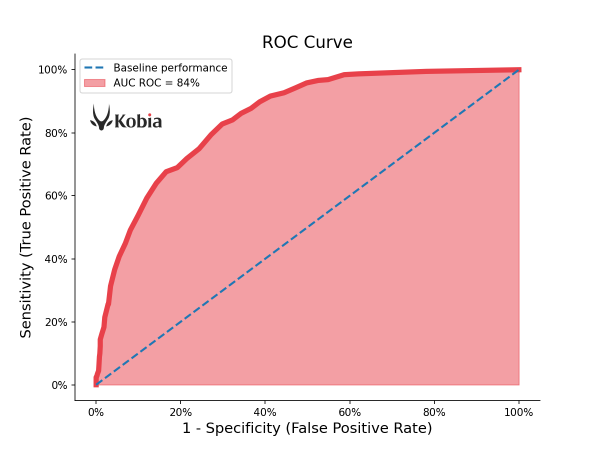
\includegraphics[width=0.7\textwidth,height=0.3\textheight]{AUC_ROC_application.png}
    \caption{Exemple d'une courbe ROC}\cite{classification_metrics_auc_roc}
    \label{fig:example24}
    \end{figure}
    \\
    tel que les facteurs nécessaires pour résulter cette courbe sont calculés de la manière suivante : \\
    \begin{figure}[htbp]
    \centering
    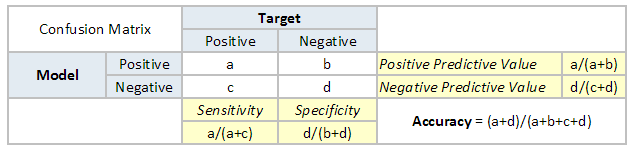
\includegraphics[width=0.8\textwidth,height=0.2\textheight]{ROC_facteurs.png}
    \caption{Calculs des facteurs du courbe AUC ROC\cite{important_model_evaluation_error_metrics}}
    \label{fig:example25}
    \end{figure}

    
\item \textbf{Perte (Loss)} : C'est une mesure utilisée pendant l’entraînement du modèle. Des fonctions de perte telles que l’entropie croisée binaire ou l’erreur quadratique moyenne sont couramment utilisées.


\item \textbf{Erreur quadratique moyenne}
C'est la moyenne des carrés des différences entre les prédictions du modèle et les valeurs réelles. Il existe aussi l'erreur logarithmique quadratique moyenne , les deux sont utilisées dans les modèles de régression.

\item \textbf{Entropie croisée (Cross-entropy)}
Dans les tâches de classification, nous traitons des prédictions de probabilités, ce qui signifie que la sortie d'un réseau neuronal doit être comprise entre zéro et un. Une fonction de perte capable de mesurer l'erreur entre une probabilité prédite et l'étiquette qui représente la classe réelle est appelée fonction de perte d'entropie croisée.
\begin{figure}[htbp]
    \centering
    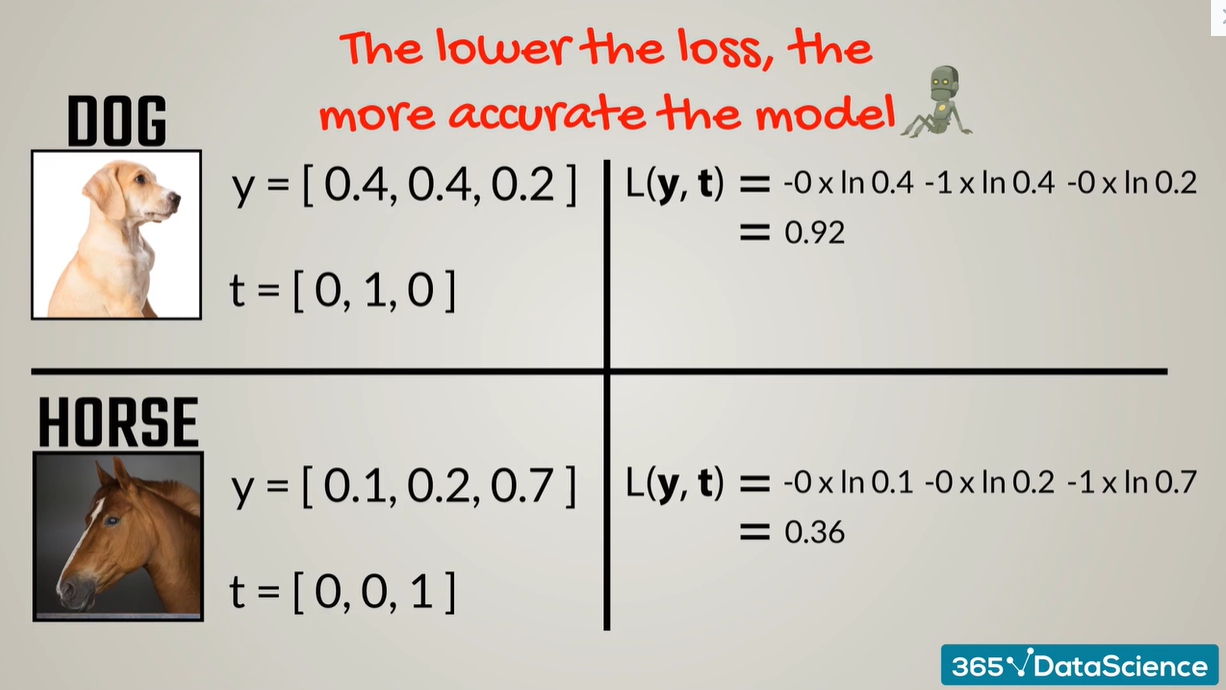
\includegraphics[width=0.6\textwidth,height=0.2\textheight]{cross_entropy_example.png}
    \caption{Exemple illustratif du déroulement de la fonction de perte "entropie croisée"\cite{cross_entropy_loss}}
    \label{fig:example26}
    \end{figure}
Une chose importante dont nous devons discuter avant de continuer avec l'entropie croisée est de savoir à quoi ressemble exactement le vecteur de vérité terrain dans le cas d'un problème de classification.

Le vecteur d'étiquette t est codé soit zéro soit un (soit le modèle a prédit l'objet/classe i (1) ou non(0) ).

La prédiction y peut cependant prendre des valeurs continues comprises entre zéro et un , car ils sont des probabilités que l'élément d'entrée soit de tel classe (pour chaque classe) .

Étant donné le vecteur de prédiction Y et le vecteur de vérité terrain Ŷ, vous pouvez calculer la perte d'entropie croisée entre ces deux vecteurs comme suit :

    \begin{figure}[htbp]
    \centering
    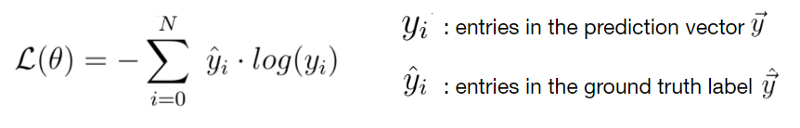
\includegraphics[width=0.5\textwidth,height=0.05\textheight]{loss_functions.png}
    \caption{Fonction de perte "Entropie croisée"\cite{loss_functions}}
    \label{fig:example27}
    \end{figure}


\item \textbf{R-carré/R-carré ajusté}
C'est une métrique statistique utilisée pour évaluer la qualité d'ajustement d'un modèle de régression.
\end{itemize}
\subsection{Conclusion}
En conclusion , la globalité des techniques de l'intelligence artificielle (que ça soit de l'IA ou le machine learning ou le deep learning) ont réussi à résoudre n'importe sorte de problème , simple ou compliqué